% $Author: Benjamin $
% $Date: 2012-01-21 02:28:33 +0200 $
% $Revision: 28563 $



%=================================================================
\ifx\wholebook\relax\else
% --------------------------------------------
% Lulu:
	\documentclass[a4paper,10pt,twoside]{book}
	\usepackage[
		papersize={6.13in,9.21in},
		hmargin={.75in,.75in},
		vmargin={.75in,1in},
		ignoreheadfoot
	]{geometry}
	\usepackage{xspace}

	\input{./common.tex}
	\setboolean{lulu}{true}
    \newcommand{\cb}[1]{\nnbb{Camillo}{#1}} % Camillo Bruni
    \newcommand\nautilus{\emph{Nautilus}\xspace}
% --------------------------------------------
% A4:
%	\documentclass[a4paper,11pt,twoside]{book}
%	\input{../common.tex}
%	\usepackage{a4wide}
% --------------------------------------------
    \graphicspath{{figures/} {./figures/}}
	\begin{document}
	
\fi
%=================================================================
%\renewmessage{\nnbb}[2]{} % Disable editorial comments
\sloppy
%=================================================================


\chapter{Nautilus}


\nautilus is a new browser made on top of Morphic. It was designed to browse \emph{RPackage}, to be compatible with the RB refactoring engine, to be \emph{environment aware} and to work with Announcements.

Quite a while ago it became obvious that a lot of needed features were missing in the current browsers. So we decided to make the new browser as simple as possible to extend and at the same time complete enough to become a really helpful environment.

\begin{center}
	\includegraphics[width=10cm]{figures/nautilus1}
	\label{fig:nautilus1}
\end{center}


\section{Main Features}

In this section the main features of \nautilus will be explained but keep in mind that there are a lot of little tricks which make \nautilus nice to work with.

\subsection*{RPackage}

\emph{RPackage} is a  model for packages. So instead of having to parse Strings and so on, you can manipulate real objects and query them about the system. \nautilus is the default browser to navigate through \emph{RPackages}.

\subsection*{Environment aware}

We wanted \nautilus to be able to be easily connected with the refactoring engine. This way we made \nautilus totally dependent of a unique entry point which is an environment. So the whole system builds queries through this entry point. It enables browsing specific environments as remote systems or different name spaces.

\subsection*{Ring}

Using the same logic we decided to make \nautilus \emph{Ring compliant}. This way we ensure that you can browse every piece of code using the tool. In addition to the sources in the image \nautilus together with \emph{Ring} can browse change sets, slice, method references etc.

\subsection*{Announcements}

Since \emph{Announcements} are used by \emph{RPackage} and should replace Events soon, we have choose to only use \emph{Announcements} in \nautilus. Currently the following \emph{Announcements} are generated:
\begin{itemize}
    \item when the system is modified and notify the changes
	\item when \nautilus emits its own changes (for plugins by example)
\end{itemize}

\subsection*{Groups}

We have noticed that most of the time when you are working your modifications are focussed on 2 or 3 packages. However in the default browser these packages are hidden in the list of all packages. Hence we have created groups to 
\begin{itemize}
	\item select only the packages you are interested in
	\item join classes from different packages in single place
	\item be able to hide the information irrelevant to your task.
\end{itemize}
\begin{center}
	\includegraphics[width=10cm]{figures/group1}
	\label{fig:group1}
\end{center}

\subsection*{Multi-Selections}

We found out that most of the time the actions you are doing when manipulating the infrastructure are the same for a set of objects. By example when you refactor a class, you move a set of methods from a protocol to another. And this kind of example is relevant at different levels of the hierarchy. Hence we implemented multi-selection lists to be able to do such manipulations at once.
\begin{center}
	\includegraphics[width=10cm]{figures/multiSelection1}
	\label{fig:multiSelection1}
\end{center}

\subsection*{Shortcuts}

Because we do not want to be forced to use the mouse to navigate through the browser while coding and because it breaks the working flow, a lot of shortcuts have been implemented to increase the efficiency of the developer while using \nautilus.

The full list of shortcuts is available in the section~\ref{sec:shortcuts}. 

\subsection*{Interactive Icons}

We were looking for a way to provide more information about the different structures. Then we realized that icons on list elements could provide those information at a glance. Thanks to that, you can instantly know that the method you are reading comes from a trait. Or that it is overriding a method from a superclass. And then we wanted to go further by providing an interaction with the icons, therefore most of the icons can be clicked. 

See the section~\ref{sec:icons} for the complete list of icons.
\begin{center}
	\includegraphics[width=10cm]{figures/icons1}
	\label{fig:icons1}
\end{center}


\subsection*{Plugins}

One of our goals was to make \nautilus easily extendable. To reach this goal we implemented a plugin mechanism. Every external project can create a \emph{Nautilus-Plugin} and then the user can plug it into his browser, or the project can register the plugin to be loaded by default. 

Each plugin can have an optional graphical part included into \nautilus and listen to \emph{Announcements} emitted by \nautilus.

Read the section~\ref{sec:plugins} to learn how to create your own plugin.

\begin{figure}[ht]
\begin{center}
	\includegraphics[width=5cm]{figures/plugin1}
	\label{fig:plugin1}
	\includegraphics[width=5cm]{figures/plugin2}
	\label{fig:plugin2}
\end{center}
\begin{center}
	\includegraphics[width=10cm]{figures/plugin3}
	\label{fig:plugin3}
\end{center}
\end{figure}
\newpage

\subsection*{Extendable menus}

Always with the idea of being easily extendable, all the menus of \nautilus are defined using pragmas. This allows every external package to create an extension possibly adding entries to menus as long as it links the method to the correct pragma(s).

\section{Shortcuts}\label{sec:shortcuts}
\subsection{Packages}

%	aCharacter == $b ifTrue: [ ^ self fullBrowse ].
%	aCharacter == $B ifTrue: [ ^ self restrictedBrowsePackage ].
%	aCharacter == $e ifTrue: [ ^ self addPackageInGroup ].
%	aCharacter == $f ifTrue: [ ^ self findClass ].
%	aCharacter == $F ifTrue: [ ^ self findPackage ].
%	aCharacter == $g ifTrue: [ ^ self addPackageAsGroupAndBrowse ].
%	aCharacter == $G ifTrue: [ ^ self addPackageAsGroups ].
%	aCharacter == $m ifTrue: [ ^ self addMatchingPackagesInGroupsAndBrowse ].
%	aCharacter == $M ifTrue: [ ^ self addMatchingPackagesInGroups ].
%	aCharacter == $n ifTrue: [ ^ self addPackage ].
%	(aCharacter == $r and: [ self enableSingleMenuItems ]) ifTrue: [ ^ self renamePackage ].
%	aCharacter == $t ifTrue: [ ^ self runPackagesTests ].
%	aCharacter == $x ifTrue: [ ^ self removePackage ].

\begin{tabular}{l | l | l}
Shortcut & Effect & Selection\\
\hline
\hline
\verb?Cmd+b? & Open a new browser browsing the same objects & Unique\\
\hline
\verb?Cmd+B?& Open a new browser browsing an environment & Multiple\\
 &based on the selected packages & \\
\hline
\verb?Cmd+e? & Add the selected packages in a group& Multiple\\
\hline
\verb?Cmd+f? &  Search for a class& None\\
\hline
\verb?Cmd+F? & Search for a package& None\\
\hline
\verb?Cmd+g? & Create groups based on the selected packages & Multiple\\
&and browse them&\\
\hline
\verb?Cmd+G? & Create groups based on the selected packages&Multiple\\
\hline
\verb?Cmd+m? & Create groups based on the packages whose & Unique\\
        & name match the selected package and browse it &  \\
\hline
\verb?Cmd+n? & Create a new package&None\\
\hline
\verb?Cmd+r? & Rename a package&Unique\\
\hline
\verb?Cmd+t? & Run tests for selected packages&Multiple\\
\hline
\verb?Cmd+x? & Remove selected packages&Multiple\\
\hline
\end{tabular}

\subsection{Groups}

%	aCharacter == $b ifTrue: [ ^ self fullBrowse ].
%	aCharacter == $B ifTrue: [ ^ self restrictedBrowseGroup: self selectedGroups ].
%	aCharacter == $f ifTrue: [ ^ self findClass ].
%	(aCharacter == $r and: [ self enableSingleMenuItems ]) ifTrue: [ ^ self renameGroup ].
%	aCharacter == $t ifTrue: [ ^ self runTestsOfGroups: self selectedGroups ].
%	aCharacter == $x ifTrue: [ ^ self removeGroup ].

\begin{tabular}{l | l | l}
Shortcut & Effect & Selection\\
\hline
\hline
\verb?Cmd+b? & Open a new browser browsing the same objects & Unique\\
\hline
\verb?Cmd+B?& Open a new browser browsing an environment & Multiple\\
 &based on the selected groups & \\
\hline
\verb?Cmd+f? &  Search for a class& None\\
\hline
\verb?Cmd+r? & Rename a group&Unique\\
\hline
\verb?Cmd+t? & Run tests for selected groups&Multiple\\
\hline
\verb?Cmd+x? & Remove selected groups&Multiple\\
\hline
\end{tabular}

\subsection{Classes}

%	aCharacter == $b ifTrue: [ ^ self fullBrowse ].
%	aCharacter == $B ifTrue: [ ^ self restrictedBrowseClass ].
%	aCharacter == $c ifTrue: [ ^ self copyClass ].
%	aCharacter == $e ifTrue: [ ^ self addClassInGroup ].
%	aCharacter == $f ifTrue: [ ^ self findMethod ].
%	aCharacter == $F ifTrue: [ ^ self findClass ].
%	aCharacter == $I ifTrue: [ ^ self generateInitialize ].
%	(aCharacter == $j and: [ self enableSingleClassSelection ]) ifTrue: [ self createTestForSelectedClass ].
%	aCharacter == $K ifTrue: [ ^ self forceGenerateInitialize ].
%	aCharacter == $N ifTrue: [ ^ self browseClassRefs ].
%	aCharacter == $n ifTrue: [ ^ self addClass ].	
%	(aCharacter == $r and: [ self enableSingleClassSelection ]) ifTrue: [ ^ self renameClass ].
%	aCharacter == $t ifTrue: [ ^ self runClassTests ].
%	aCharacter == $x ifTrue: [ ^ self removeClasses ].

\begin{tabular}{l | l | l}
Shortcut & Effect & Selection\\
\hline
\hline
\verb?Cmd+b? & Open a new browser browsing the same objects & Unique\\
\hline
\verb?Cmd+B?& Open a new browser browsing an environment & Multiple\\
 &based on the selected classes & \\
\hline
\verb?Cmd+c?& Copy the selected classes & Multiple \\
\hline
\verb?Cmd+e?& Add classes in a group & Multiple \\
\hline
\verb?Cmd+f?& Find a method in the selected package & None \\
\hline
\verb?Cmd+F?& Find a class & None \\
\hline
\verb?Cmd+I?& Generate a initialize method for & Unique \\
&the selected class&\\
\hline
\verb?Cmd+j?& Create a class test for the selected class & Unique \\
\hline
\verb?Cmd+K?& Force the generation of a initialize method & Unique \\
&for the selected class &\\
\hline
\verb?Cmd+N?& Browse the references to the selected class & Unique \\
\hline
\verb?Cmd+n?& Add a class & None \\
\hline
\verb?Cmd+r?& Rename the selected class & Unique \\
\hline
\verb?Cmd+t?& Run the tests for the selected classes & Multiple \\
\hline
\verb?Cmd+x?& Remove the selected classes & Multiple \\
\hline
\end{tabular}

\subsection{Protocols}

%	aCharacter == $b ifTrue: [ ^ self model  fullBrowse ].
%	aCharacter == $f ifTrue: [ ^ self model  findMethod ].	
%	aCharacter == $n ifTrue: [ ^ self model  addCategory ].
%	(aCharacter == $r and:[ self model  enableCategorySingleSelection ]) ifTrue: [ ^ self model  renameCategory ].
%	aCharacter == $x ifTrue: [ ^ self model  removeCategories ].	

\begin{tabular}{l | l | l}
Shortcut & Effect & Selection\\
\hline
\hline
\verb?Cmd+b? & Open a new browser browsing the same objects & Unique\\
\hline
\verb?Cmd+f? & Find a method in the selected class & None\\
\hline
\verb?Cmd+n? & Create a new protocol & None\\
\hline
\verb?Cmd+r? & Rename a protocol & Unique\\
\hline
\verb?Cmd+x? & Remove the selected protocols & Multiple\\
\hline
\end{tabular}

\subsection{Methods}

%	aCharacter == $b ifTrue: [ ^ self model fullBrowse ].
%	aCharacter == $C ifTrue: [ ^ self model categorizeMethod ].
%	aCharacter == $f ifTrue: [ ^ self model findMethod ].
%	(aCharacter == $i and:[ self model enableMethodSingleSelection ]) ifTrue: [ ^ self model methodHierarchy ].
%	(aCharacter == $j) ifTrue: [ ^ self model generateTestMethodsAndFocus: true ].
%	(aCharacter == $J) ifTrue: [ ^ self model generateTestMethodsAndFocus: false ].
%	(aCharacter == $m and:[ self model enableMethodSingleSelection ]) ifTrue: [ ^ self model browseMessages ].
%	(aCharacter == $n and:[ self model enableMethodSingleSelection ])	ifTrue: [ ^ self model browseSendersOfMessages ].		
%	(aCharacter == $t) ifTrue: [ ^ self model runTestFor: self selectedMethods ].
%	(aCharacter == $v and:[ self model enableMethodSingleSelection ]) ifTrue: [ ^ self model browseVersions ].
%	aCharacter == $x ifTrue: [ ^ self model removeMethods ].

\begin{tabular}{l | l | l}
Shortcut & Effect & Selection\\
\hline
\hline
\verb?Cmd+b? & Open a new browser browsing the same objects & Unique\\
\hline
\verb?Cmd+C? & Re-categorize the selected methods & Multiple\\
\hline
\verb?Cmd+f? & Find a method in the selected class & None\\
\hline
\verb?Cmd+i? & Display the selected method hierarchy & Unique\\
\hline
\verb?Cmd+j? & Generate a test method for each selected& Multiple\\
& methods and browse them&\\
\hline
\verb?Cmd+J? & Generate a test method for each & Multiple\\
&selected methods&\\
\hline
\verb?Cmd+m? & Browse implementors of the selected  & Unique\\
&method selector&\\
\hline
\verb?Cmd+n? & Browse the senders of the selected & Unique\\
&method selector &\\
\hline
\verb?Cmd+t? & If the selected methods are tests one, tun them & Multiple\\
\hline
\verb?Cmd+v? & Browse versions of the selected method & Unique\\
\hline
\verb?Cmd+x? & Remove the selected methods& Multiple\\
\hline
\end{tabular}
\section{Icons}\label{sec:icons}

\subsection{Packages}
\begin{tabular}{l | l | l}
Icon & Meaning & If clicked\\
\hline\hline
\raisebox{-1.5ex}{
\includegraphics[width=20px]{figures/Package}} & The default package icon& Can't be clicked\\
\raisebox{-1.5ex}{\includegraphics[width=20px]{figures/DirtyPackage}} & The corresponding MCPackage is dirty& Open the MonticelloBrowser\\
&& on this package\\
\raisebox{-1.5ex}{\includegraphics[width=20px]{figures/EmptyPackage3}} & The package is empty& Can't be clicked\\
\end{tabular}

\subsection{Groups}
\begin{tabular}{l | l | l}
Icon & Meaning & If clicked\\
\hline\hline
\raisebox{-1.5ex}{\includegraphics[width=20px]{figures/Cube2}} & The default group icon& Open a new browser browsing an environment\\
& &based on the selected classes \\
\end{tabular}

\subsection{Classes}

\begin{tabular}{l | l | l}
Icon & Meaning & If clicked\\
\hline\hline
\raisebox{-1.5ex}{\includegraphics[height=20px]{figures/UncommentedClass}} & The class is not commented& Pop up a comment editor\\
\raisebox{-2.8ex}{\includegraphics[width=20px]{figures/Gray}} & The tests haven't been run& Run the tests\\
\raisebox{-2.8ex}{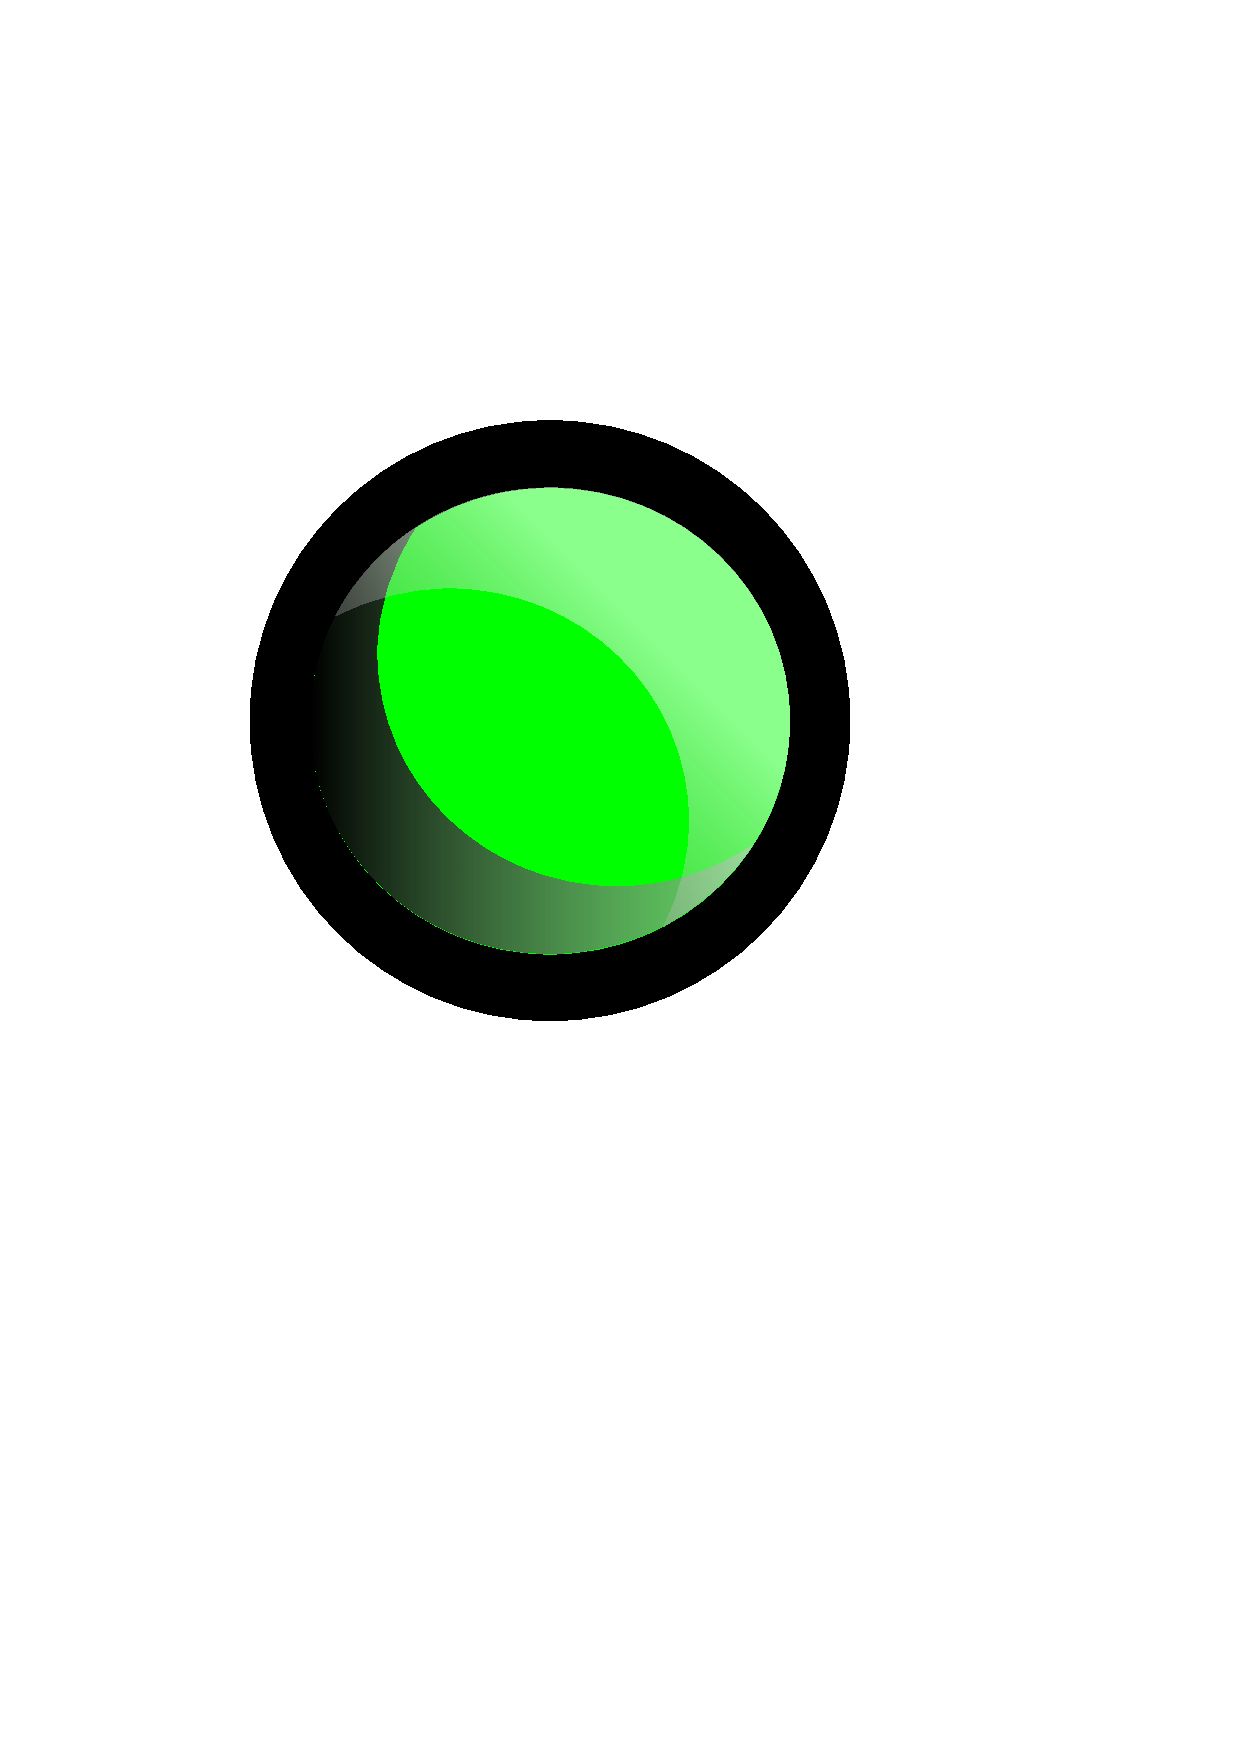
\includegraphics[width=20px]{figures/Green}} & The tests passed & Run the tests\\
\raisebox{-2.8ex}{\includegraphics[width=20px]{figures/Yellow}} & Some of the tests failed & Run the tests\\
\raisebox{-2.8ex}{
\includegraphics[width=20px]{figures/Red}} & Some of the tests produced an error & Run the tests\\
\end{tabular}

\subsection{Protocols}

For the moment, there is no icons on protocols.

\subsection{Methods}
\begin{tabular}{l | l | l}
Icon & Meaning & If clicked\\
\hline\hline
\raisebox{-2.8ex}{\includegraphics[width=20px]{figures/ArrowUp}} & The method overrides another method & Jump to the overridden method\\
\raisebox{-2.8ex}{\includegraphics[width=20px]{figures/ArrowDown}} & The method is overridden& Browse the methods\\
\raisebox{-2.8ex}{\includegraphics[width=20px]{figures/Trait}} & The method comes from a trait & Browse the Trait class\\
\raisebox{-2.8ex}{\includegraphics[width=20px]{figures/Gray}} & The test has not been run& Run the test\\
\raisebox{-2.8ex}{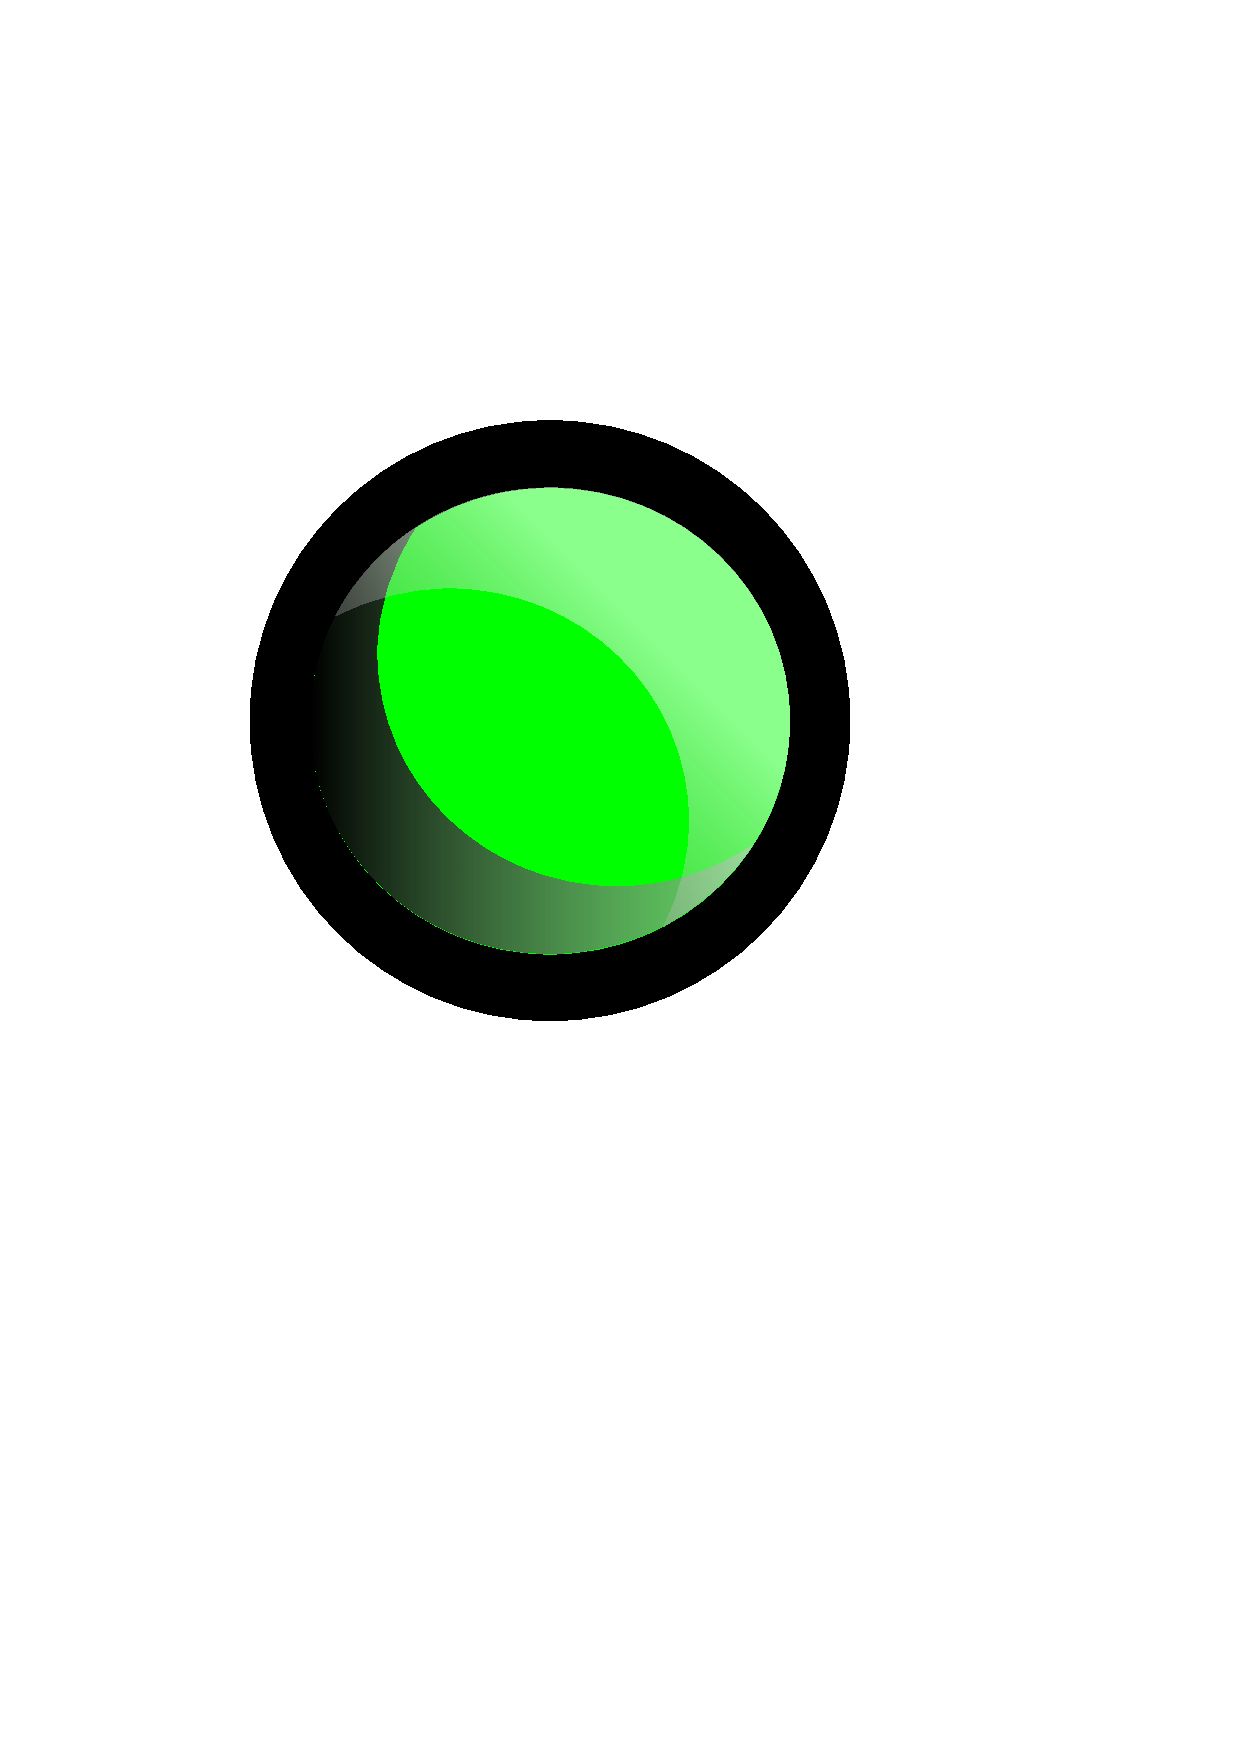
\includegraphics[width=20px]{figures/Green}} & The test passed & Run the test\\
\raisebox{-2.8ex}{\includegraphics[width=20px]{figures/Yellow}} & The test failed & Run the test\\
\raisebox{-2.8ex}{
\includegraphics[width=20px]{figures/Red}} & The test produced an error & Run the test\\
\end{tabular}



\section{How to create Nautilus-Plugins}\label{sec:plugins}

Here we will give some brief explanations on how to create your own plugin.
By the way there are only two requirements to create a \emph{Nautilus-Plugin}:
\begin{itemize}
	\item the class should inherit from \verb?AbstractNautilusPlugin?
	\item it should implement \verb?#registerTo: aModel?
\end{itemize}


\subsection{Announcement subscription}

The method \verb?#registerTo:? is used by the plugin to register itself to \verb?aModel? announcements.

\begin{code}{Example of #registerTo:}
MyPlugin>>#registerTo: aModel

	aModel announcer
		on: NautilusKeyPressed send: #keyPressed: to: self
\end{code}
In this example, the instance of \verb?MyPlugin? subscribe themselves to \verb?NautilusKeyPressed?, and tell \emph{aModel's announcer} to send: \verb?#keyPressed? to the instance.

So each time a key will be pressed in a Nautilus window the method \verb?keyPressed:? will be called.

\subsection{Display}

If you want your plugin to add a graphical widget to \nautilus you should override the \verb?display? method. This method should return the \emph{Morphic} element you want \nautilus to display. By default the method returns nil to notify \nautilus not to display anything.

\begin{code}{Example of #display}
MyPlugin>>#display

	morph :=  LabelMorph new 
					contents: '';
					enabled: false;
					vResizing: #shrinkWrap;
					hResizing: #spaceFill;
					yourself.
	^ morph
\end{code}

You can also redefine the following methods on the class side:
\begin{itemize}
	\item \verb?#defaultPosition? : defines the default position of the morph (possible values are \{\#top, \#middle, \#bottom, \#none\}). The default value is \#none.
	\item \verb?#possiblePositions? : answers a collection of the possible positions the widget could adopt.
\end{itemize}

And finally you could redefine the \verb?name? method to change the name displayed in the \emph{Nautilus Plugin Manager}.

\end{document}
